% !TeX document-id = {a7325568-63cb-46d1-95d6-777a45054e5a}
% !TeX TXS-program:compile = txs:///pdflatex/[--shell-escape]
\documentclass{article}
\usepackage{style}
\begin{document}
\maketitle
\tableofcontents
\section{Introducción}
La célula de McCulloch-Pitts fue el primer modelo de un neurona biológica como un dispositivo de dos estados:
\begin{itemize}
	\item Apagado(0)
	\item Encendido(1)
\end{itemize}
Es la unidad escencial con la cual se construye una red neuronal artificial\\
En esta práctica usaremos un modelo similar a este ya que el umbral no se aplica a la suma, si no que es parte de la función de activación. Usaremos aprendizaje supervisado ya que $\forall$ conjunto de valores $v$ $\exists$ un target $t$
\subsection{Modelo}
\begin{figure}[h!]
	\caption{Modelo}
	\centering
	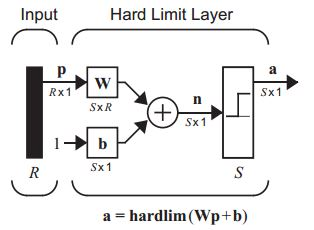
\includegraphics{model}
\end{figure}
Donde $x_1, x_2,\ldots, x_n$ son los valores de entrada, $w_1, w_2,\ldots, w_n$ son los pesos sinápticos, $\theta$ es un valor de umbral que se usa para activar la señal de entrada.\\
Matemáticamente podemos representar esta célula con las siguientes expresiones:\\
\begin{align}
	n &= \sum_{i=1}^{R}W_i*P_i
\end{align}
\begin{align}
	s &{}=\displaystyle
	\begin{cases}
		1 &\text{si } n > \theta\\
		0 &\text{en otro caso}
	\end{cases}
\end{align}
\newpage
\section{Diagrama de Flujo}
\begin{figure}[htpb]
	\centering
	\includesvg[width = 400pt, height = 400pt]{diagram}
	\caption{Diagrama de Flujo}
\end{figure}
\section{Fórmula general para las compuertas AND y OR}
Debido a que trabajamos con valores lógicos se propone que los pesos sinápticos siempre sean unos.
\subsection{AND}
La única forma de que la salida de esta sea ``1'' es que todas las entradas sean ``1's', entonces $n=w_1*p_1 + w_2*p_2 + \ldots + w_n*p_n$ se puede simplificar a $n = tam(w)$, por lo tanto, n tiene que ser mayor al umbral solo en ese caso, entonces, el umbral sería $\theta = tam(w) - 1$.\\
Explicado matemáticamente para cuando la salida de AND es 1:\\
$ p = (p_1, p_2, \ldots, p_r) = (1, 1, \ldots, 1)$\\
$ w = (w_1, w_2, \ldots, w_r) = (1, 1, \ldots, 1)$\\
$ r > 0$\\
$ n = w_1*p_1 + w_2*p2, + \ldots +w_r*p_r = tam(w)$\\
$ f(n) = 1 \rightarrow (n > \theta)$\\
$ \therefore \theta = tam(w) - 1$
\subsection{OR}
La única forma en que la salida sea '0' es que todas las entradas sean '0', entonces $ n=w_1*p_1 + w_2*p_2 + \ldots + w_n*p_n$ se puede simplificar a $ n = 0$. n tiene que ser mayor al umbral para todos los demás casos, entonces el umbral sería 0.\\
Explicado matemáticamente para cuando la salida de OR es 0:\\
$ p = (p_1, p_2, \ldots, p_r) = (0, 0, \ldots, 0)$\\
$ w = (w_1, w_2, \ldots, w_r) = (1, 1, \ldots, 1)$\\
$ r > 0$\\
$ n = w_1*p_1 + w_2*p2, + \ldots +w_r*p_r = 0$\\
$ f(n) = 0 \rightarrow (n \leq \theta)$\\
Dejando a un lado a los enteros negativos: $\theta = 0$
\section{Resultados}
\subsection{Compuerta NOT}
\subsection{Compueta AND}
\subsection{Compuerta OR}
\section{Discusión de Resultados}
\section{Referencias}
D. Michie, D.J. Spiegelhalter, C.C. Taylor (eds). Machine Learning, Neural and Statistical Classification, 1994.\\
Apuntes de Doctor Marco Antonio Moreno Armendáriz
\section{Apéndice}
\begin{lstlisting}[
style=Matlab-editor,
basicstyle=\mlttfamily,
escapechar=`,
caption={Código},
]
% User input
gate = input('Ingrese la compuerta (and, or, not): ', 's');
syn_prompt = 'Ingrese el valor de los pesos sinapticos separados por espacios
(e.g. 1 2 3 4): ';
w = str2num(strip(input(syn_prompt, 's')));
theta = input('Ingrese el valor del umbral: ');
if (gate == "not" && size(w, 2) > 1)
	fprintf("Error, la compuerta NOT es de una sola entrada");
else
	% Generation of table for inputs and targets
	model = logicalModel(size(w, 2), gate)
	error = false;
	% Iteration process
	for i = 1:size(model, 1)
		row = model(i, :);
		% Calculation of n
		n = sum(row(1:end-1).*w);
		% Calculation of a
		if(n > theta); a_n = 1; else; a_n=0; end
			% Comparison between a and the threshold
			fprintf("n_%i = %i -> t_%i = %i\n", i, a_n, i, row(end));
			if(a_n ~= row(end)); error = true; break; end
	end
		if(~error); fprintf("El aprendizaje fue exitoso\n"); 
		else; fprintf("El aprendizaje no fue exitoso\n"); end
end


function [table] = logicalModel(i, gate)
	% logicalModel(I, gate) returns a matrix representing a truth table and
	% the last column represents the oupot base on all the previous columns
	% based on the (gate) parameter
	% INPUT: (I) shall be an integer >= 1
	% INPUT: (gate) shall be 'and' or 'or'
	% OUTPUT: logicalModel is a binary matrix of size [2^I,I + 1]
	% Heavily inspired in Paul Metcalf's CONDVECTS
	% Acknowledgements: Paul Metcalf

	g = 2;
	i2 = 2^i;
	table = false(i2,i + 1);
	for m = 1 : 1 : i
		m2 = 2^m;
		m3 = (m2/2)-1;
		i3 = i-m+1;
		for g = g : m2 : i2
			for k = 0 : 1 : m3
				table(g+k,i3) = true;
			end
		end
		g = m2+1;
	end
	if (gate == "and")
		for row_index = 1:size(table, 1)
			row = table(row_index,:);
			res = row(1);     
			for e_index = 1:size(row, 2)-1
				res = res & row(e_index);
			end
			table(row_index, end) = res; 
		end  
	elseif (gate == "or")
		for row_index = 1:size(table, 1)
			row = table(row_index,:);
			res = row(1);     
			for e_index = 1:size(row, 2)-1
				res = res | row(e_index);
			end
			table(row_index, end) = res; 
		end 
	elseif (gate == "not")
		for row_index = 1:size(table, 1)
			row = table(row_index,:);
			res = ~row(1);     
			table(row_index, end) = res; 
		end
	end  
end
\end{lstlisting}
\end{document}